\section{Scalable Polygon Extraction for Line-based Input} \label{sec:polygonization}

Our discussion so far assumed the input data is a set of clean and closed polygons in the two input layers to be overlayed. However, several real-world 
polygons, such as city blocks formed by individual road segments represented as spatial lines, are unavailable in the polygonal form. Forming polygons in such 
cases at a large scale is non-trivial and takes significant computing cost. This section further extends our scalable DCEL overlay operations to handle 
scattered line segments as input through a scalable polygonization \cite{abdelhafeez_ddcel_2023} process. Such a feature enables spatial data scientists to 
seamlessly  
exploit a rich set of publicly available datasets, e.g., spatial road networks worldwide \cite{web:data:continents,web:data:usa}.

\begin{figure}[tb]
	\centering
	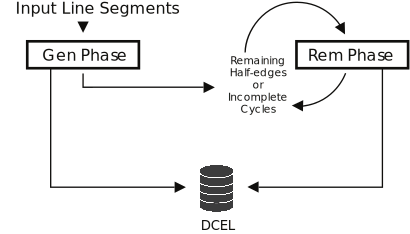
\includegraphics[width=0.75 \linewidth ]{chapterSDCEL/model/overview_updated.png}
	\caption{DCEL Constructor for Polygonization Overview}
	\label{fig:overview_ddcel}
\end{figure}

Building a DCEL data structure from an input of planar line segments extracts all closed polygons during the invocation of the \textit{polygonization} 
procedure.  In our work in \cite{abdelhafeez_ddcel_2023}, we proposed a scalable distributed framework to build a DCEL and extract polygons in parallel from 
the 
input 
line segments. Figure \ref{fig:overview_ddcel} shows an overview of the DCEL constructor. 

To create a DCEL data structure from input line segments, the \textit{DCEL constructor} undergoes a two-phase paradigm.  The \textit{Gen Phase}, detailed in 
Section \ref{sec:gen}, spatially partitions the input lines, generating the subdivision's vertices ($V$) and half-edges ($H$), and a subset of the 
subdivision's faces ($F_0$). 

The remaining line segments that are not assigned to a face yet are passed to the subsequent phase in the form of half-edges or incomplete cycles. An 
incomplete 
cycle is a connected half-edge list that is a candidate face. The \textit{Rem Phase}, detailed in Section \ref{sec:rem}, generates the subdivision's remaining 
faces, $F_j, \ \forall j > 0$. 

Section \ref{sec:partitioning_ddcel} discusses different data re-partitioning schemes with a minimal number of iterations to reduce the workload of the 
\textit{Rem Phase} without compromising correctness. The polygonization procedure produces two outputs: first, a set of closed polygons formed by the input 
planar line segments, and second, any edges that are not a part of any polygon, i.e., dangle or cut edges. Overlaying the polygons generated with any polygon 
layer follows the approaches discussed in sections \ref{sec:methods}and \ref{sec:alternative_methods}. In section \ref{sec:over_dang}, we extend the overlay 
approaches to handle overlaying a polygon layer with the remaining edges (the dangle and cut edges).

\subsection{Gen Phase}
\label{sec:gen}

The Gen phase accepts an input dataset of line segments $N$ and starts by partitioning the input across the worker nodes in a distributed cluster using a global quadtree spatial index.
Each data partition $P_i$ covers a specific spatial area represented by its minimum bounding rectangle (MBR) $B_i$.
Figure~\ref{fig:ddcel:input} shows an example of four leaf nodes of a quadtree built for input spatial line segments. Solid lines represent the line segments, and dashed lines represent the partitions' MBRs.

\begin{figure}[tb]
	\centering
	\includegraphics[width=0.75 \linewidth ]{chapterSDCEL/model/input-network}
	\caption{Partitioned input spatial lines.}
	\label{fig:ddcel:input}
\end{figure}

After spatially partitioning the input lines, each partition generates its vertices, half-edges, and faces (collectively the partition DCEL) using the subset of 
the dataset that intersects with the partition's MBR.
The \textit{partition vertices} are the vertices that are wholly contained within the partition MBR. 
On the other hand, the \textit{partition half-edges} are any half-edge that intersects with the partition MBR.
\textit{Partition faces} are the faces that are wholly contained within the MBR of the partition.
On each data partition $P_i$, the Gen phase undergoes four main procedures; 
(1) first, generating the partition vertices and half-edges, 
(2) second, marking the dangle half-edges, 
(3) third, setting the next half-edge pointers for all half-edges and marking the cut edges, 
(4) lastly, generating the partition faces. 

\vspace{4pt}
\textit{\textbf{Step 1: Generating the Partition Vertices and Half-edges.}}
\\
In the first step, the Gen Phase starts with populating the vertices and the half-edges RDDs of the DCEL data structure.
Each partition $P_i$ receives a subset of the input dataset that intersects with the partition's boundary.
For every line segment object $o$ received at partition $P_i$ ($o \in P_i$), two vertices are generated ($v_1$, $v_2$); one for each endpoint on this line 
segment ($p_1$, $p_2$). These two vertices objects ($v_1, v_2$) are appended to the vertices RDD in the DCEL data structure.
We also generate two half-edges ($h_1, h_2$) for every line segment. 
The first half-edge $h_1$ has its destination vertex $v_1$, while the other half-edge $h_2$ has its destination vertex $v_2$. These two half-edges are assigned 
as twins.
The half-edge $h_1$ is appended to the incident list of the vertex $v_1$. Similarly, $h_2$ is appended to $v_2$'s incident list.
For a half-edge to span multiple partitions, we check whether it is wholly contained within the partition MBR $B_i$; if not, and it is just intersecting, then 
this half-edge spans multiple partitions. 
These half-edges are duplicated on all partitions they intersect with.
The remaining attributes of each half-edge object are assigned in the subsequent steps. 
The two generated half-edge objects ($h_1, h_2$) are appended to the half-edges RDD in the DCEL data structure.
Figure \ref{fig:ddcel:step1} shows a graphical illustration of the DCEL data structure representing the input lines after generating the vertices and the 
half-edges on all data partitions.

\begin{figure}[tb]
	\centering
	\includegraphics[width=0.75 \linewidth ]{chapterSDCEL/model/ddcel-1}
	\caption{DCEL vertices and half-edges.}
	\label{fig:ddcel:step1}
\end{figure}


\vspace{4pt}
\textit{\textbf{Step 2: Marking the Dangle Half-edges.}}
\\
Dangle half-edges are not part of any face; thus, marking them is essential to exclude them during the polygonization procedure. To find dangles in the input 
lines, we use previously generated information, i.e., information about the vertices and their incident half-edges. 
We compute the degree of each vertex $v \in V$ populated in the previous step. A vertex degree is the number of non-dangle half-edges in its incident half-edges 
list. If the degree of an arbitrary vertex $v$ is less than or equal to 1 ($degree(v) \le 1$), then all of $v$'s incident half-edges and their twins are also 
dangle half-edges. 
Marking any new half-edge as a dangle requires recomputing the degree of the vertices connected to it. 
Thus, marking the dangle half-edges is an iterative process. After the initial run over all vertices and marking the initial dangle half-edges, we reiterate 
over the vertices to check for newly found dangle half-edges. We keep iterating until convergence when no new dangle half-edges are detected.


\vspace{4pt}
\textit{\textbf{Step 3: Setting the Half-edges' Next Pointers, and Marking the Cut Edges.}}
\\
The third step is divided into three smaller steps: (a) setting the next half-edge pointer for each half-edge, (b) marking the cut edges, and (c) updating the 
next half-edges accordingly.
To set the next pointer for each half-edge, we use information from the previous two steps, i.e., the vertices incident half-edges and the current dangle 
half-edges.
For each vertex $v \in V$, we sort its incident half-edges list in clockwise order, excluding the dangle half-edges. 
After sorting the incident half-edges list $v.incidentH$, for every pair of half-edges $v.incidentH[t]$, $v.incidentH[t+1]$ in the sorted list, we assign 
$v.incidentH[t].next$ to $v.incidentH[t+1].twin$. For the last incident half-edge in the sorted list $v.incidentH[v.incidentH.len-1]$, we assign its next 
half-edge to $v.incidentH[0].twin$.


After the initial assignment of the next half-edge pointers, we proceed with the second sub-step, marking the cut edges.
To mark the cut edges, we start our procedure at an arbitrary half-edge $h_{initial}$ and assign our $h_{current}$ half-edge pointer to it. We advance the 
$h_{current}$ pointer at each iteration to the $h_{current}$'s next ($h_{current} = h_{current}.next$), storing all visited half-edges in a list (current 
cycle). We keep advancing the $h_{current}$ pointer till we reach one of three cases.
(1) We return to the initial half-edge $h_{initial}$, which means a cycle is detected and no cut edge is detected.
(2) The half-edge $h_{current}.next$ is not available, which also means no cut edge is detected.
(3) We find $h_{current}.twin$ in the current cycle, which means that $h_{current}$ and its twin are both cut edges. 
Once we reach one of these cases, we mark all visited half-edges as such and proceed with a new arbitrary half-edge to be $h_{initial}$.
This process is terminated when all the partition half-edges are visited.

In the third sub-step, after marking all cut edges, we update the next pointers while excluding the cut edges. 
For each vertex $v \in V$, we sort its incident half-edges list in clockwise order again, now while excluding both the dangle and the cut edge half-edges.
After sorting the incident half-edges list $v.incidentH$, we re-execute the same process of the first sub-step, assigning $v.incidentH[t].next$ to 
$v.incidentH[t+1].twin$. 
Figure~\ref{fig:ddcel:step2} shows the DCEL data structure after removing the dangle and cut edges.


\begin{figure}[tb]
	\centering
	\includegraphics[width=0.75 \linewidth ]{chapterSDCEL/model/ddcel-2}
	\caption{DCEL vertices and half-edges after dangle and cut edge removal.}
	\label{fig:ddcel:step2}
\end{figure}

\vspace{4pt}
\textit{\textbf{Step 4: Generating the Partition Faces.}}
\\
Polygonization on each partition $P_i$ starts with selecting an arbitrary half-edge as our initial half-edge $h_{initial}$.
We initially assign our $h_{current}$ half-edge pointer to $h_{initial}$. We advance the $h_{current}$ pointer at each iteration to the $h_{current}$'s next 
($h_{current} = h_{current}.next$), storing all visited half-edges in a list $cycle$. We keep advancing the $h_{current}$ pointer till we reach one of the 
following cases:
(1) We return to the initial half-edge $h_{initial}$, which means that we have found a face. In this case, we add the found face $f$ to the faces collection 
$F_0$ and assign $h.incidentF = f, \;\; \forall h \in cycle$.
(2) The $h_{current}.next$ is not available, and $h_{current}$ is a half-edge that spans multiple partitions. In this case, the cycle needs more information 
from the neighboring partitions to be completed, and the current partition's data is insufficient to produce this face.
To complete this cycle, we either pass the incomplete cycle into the Rem phase (the current list $cycle$), where it collects all incomplete cycles from all 
partitions and attempts to join them to form a face. Another approach would be passing the plain half-edges in this cycle to the next phase. Both approaches are 
discussed in detail in Section~\ref{sec:rem}.
Once we finish processing this cycle, we mark all visited half-edges as such, clear the cycle, and proceed with a new arbitrary half-edge to be $h_{initial}$.
This process is terminated when all the partition half-edges are visited.
In Figure~\ref{fig:ddcel:faces}, the dotted faces are the faces generated in this phase (Gen Phase).

\begin{figure}[tb]
	\centering
	\includegraphics[width=0.75 \linewidth ]{chapterSDCEL/model/ddcel-3}
	\caption{DCEL faces.}
	\label{fig:ddcel:faces}
\end{figure}

\subsection{Rem Phase}
\label{sec:rem}

The Rem Phase accepts the remaining half-edges or incomplete cycles as input. 
To be included in the remaining half-edges set, a half-edge cannot be a dangle or a cut edge. Also, the half-edge should not have been bounded to a face yet.
An incomplete cycle is a sequence of half-edges that acts as a candidate face. This incomplete cycle could not be completed since their marginal half-edges span multiple partitions.


The Rem Phase is an iterative phase, where each iteration $j$ generates a subset of faces $F_j$. The unused input data at iteration $j$ is passed to the next iteration $j+1$.
Faces generated from the Gen phase and the Rem phase constitute the whole faces of the subdivision $F$.
In each iteration, the Rem Phase starts with re-partitioning the input data across the worker nodes using a new set of partitions.
This new set of partitions satisfies the convergence criteria; the new number of partitions ($k_j$) at iteration $j$ must be less than the number of partitions ($k_{j-1}$) at iteration $j-1$. This criterion ($k_j < k_{j-1}$) ensures there is an iteration ($m$) at which the remaining line segments are re-partitioned to one partition only, where $m$ is the total number of iterations of the Rem Phase, converging the problem into a sequential one and guaranteeing the termination of the procedure.
After the data re-partitioning, we proceed with generating a subset of the remaining faces. Two approaches are employed for the remaining faces generation, depending on the phase input data.
The first approach assumes the phase input is a set of the \underline{R}emaining \underline{H}alf-edges (RH Approach). 
While the second approach assumes the input is a set of the \underline{I}ncomplete \underline{C}ycles (IC Approach). 

\vspace{4pt}
\textit{\textbf{RH Approach: Iterate over the Remaining Half-edges.}}
\\
At each iteration $j$ and on each new data partition, a subset of the remaining half-edges is received. 
Duplicate half-edges received on one new partition are merged into a single half-edge choosing the half-edge with the available next half-edge.
We follow the same procedure of generating faces in the Gen Phase. Starting from an arbitrary half-edge as our initial half-edge $h_{initial}$, we assign our $h_{current}$ half-edge pointer initially to $h_{initial}$. We advance the $h_{current}$ pointer at each iteration to the $h_{current}$'s next ($h_{current} = h_{current}.next$), storing all visited half-edges in a list $cycle$. We keep advancing the $h_{current}$ pointer till we reach one of the following cases:
(1) We return to the initial half-edge $h_{initial}$, which means that we have found a face. In this case, we add the found face $f$ to the faces collection $F_j$ and assign $h.incidentF = f, \;\; \forall h \in cycle$.
(2) The $h_{current}.next$ is not available, and $h_{current}$ is a half-edge that is not wholly contained in the new partition MBR.
Once we finish processing this cycle, we mark all visited half-edges as such, clear the cycle, and proceed with a new arbitrary half-edge to be $h_{initial}$.
This iteration is terminated when all the remaining half-edges are visited. All half-edges that have not been assigned to any face yet are passed to the next iteration.
The Rem Phase terminates if (1) there are no more remaining half-edges, i.e., all non-dangle non-cut edge half-edges are assigned to a face, or (2) the remaining half-edges have been processed on one partition.

\vspace{4pt}
\textit{\textbf{IC Approach: Iterate over the Incomplete Cycles.}}
\\
At each iteration $j$, and on each new data partition, a subset of the incomplete cycles is received. 
Starting from an arbitrary incomplete cycle $c_{initial}$ with first half-edge $first(c_{initial})$ and last half-edge $last(c_{initial})$, where the first and last half-edges are the incomplete cycle's terminal half-edges, we search for a match $c_{match}$ in the remaining incomplete cycles such that the $last(c_{initial}) = first(c_{match})$. When a match is found, we merge the two cycles such that the $last(c_{initial})$ is now the $last(c_{match})$. We keep merging cycles till we reach one of the following cases:
(1) The $last(c_{match}) = first(c_{initial})$, which means the cycle is now completed. In this case, we add the found face $f$ to the faces collection $F_j$ and remove all incomplete cycles used from the set of the incomplete cycles.
(2) We can not find a match for the current last half-edge, and the last half-edge is not wholly contained within the new partition's MBR. In this case, the incomplete cycle needs more information from the neighboring partitions to be completed, and the current partition's data is insufficient to produce this face.
Once we finish processing this matching process, we mark all visited incomplete cycles as such and proceed with a new arbitrary incomplete cycle to be $c_{initial}$.
This iteration $j$ is terminated when all the incomplete cycles are visited. All incomplete cycles that are not completed yet are passed into the next iteration.
The Rem Phase terminates if (1) there are no more remaining incomplete cycles, i.e., all cycles have been completed, or (2) the incomplete cycles have been processed on one partition.
In Figure \ref{fig:ddcel:faces}, the hatched faces are the faces generated in the first iteration ($j=1$) of the Rem Phase.


\subsection{Data Partitioning}\label{sec:partitioning_ddcel}

The quadtree partitioner is used again to distribute the data amongst the worker nodes across the cluster. In the Gen Phase, the quadtree leaf nodes are used as the initial data partitions.
The output of the Gen Phase, whether the remaining half-edges or the incomplete cycles, is iteratively re-partitioned into new sets of partitions.
Each iteration set of partitions must satisfy the convergence criterion to ensure that the Rem Phase will terminate.
We employ the same quadtree partitioner to generate the new partitions. 
Assume we have a quadtree built on the input line segments of height $L$. 
At the Gen Phase, we use nodes at the leaf level $L$ as our initial data partitions. For each iteration $j$ in the Rem Phase, we level up in the quadtree and choose different level nodes, aside from the leaves, to be our current data partitions.  
We keep leveling up in the quadtree till we reach the root ($l=0$), which means that all data is located on only one partition (the root).
Going up in the quadtree ensures that the number of partitions at iteration $j+1$ is less than that at iteration $j$ since the number of nodes at any arbitrary level $l$ visited at iteration $j$ is more than that at level $l_{chosen}, \ \forall l_{chosen} < l$ visited at iteration $j+1$.


We always start with the leaf nodes level $L$ in the Gen Phase. Choosing which levels to visit next in each iteration $j$ is a system parameter. 
We offer different schemes for the visited quadtree levels: 
\begin{enumerate}
    \item Going directly to the root node at $l=0$ after the leaf nodes, i.e., visiting only levels L in the Gen and 0 in the Rem phases. However, the experimental evaluation shows that collecting the data after the Gen phase on one node is prohibitive, and one worker node will not be able to process the Gen phase's output.
    \item Going \underline{1} \underline{L}evel \underline{U}p (1LU) each iteration, i.e. if we visit level $l$ at iteration $j$, we go to level $l-1$ at iteration $j+1$. This means the Rem Phase visits all the quadtree levels resulting in $L$ iterations.
    \item Going \underline{2} \underline{L}evels \underline{U}p (2LU) each iteration resulting in half the number of iterations $\frac{L}{2}$ compared to 1LU.
    \item Skipping to the \underline{M}iddle of the tree at level $\frac{L}{2}$, then continue going 1 level up for the remaining levels (M1LU), which will also result in $\frac{L}{2}$ iterations.
    \item Skipping to the \underline{M}iddle of the tree every time, dividing the current level by two each iteration (MU); this will result in $\log_2(L)$ iterations.
\end{enumerate}
The goal is to find a re-partitioning scheme with a minimal number of iterations, thus reducing the workload of the Rem Phase while ensuring that the worker nodes can process the chunk of the data it receives at each iteration $j$.
The extreme case of having only one iteration at the Rem Phase will not work since the data is too big to fit one partition and be processed by only one worker node. On the other hand, the more unnecessary iterations we have, the more overhead on the system resulting in higher query latency.


\subsection{Overlaying Polygons with Dangle and Cut Edges} \label{sec:over_dang}

\begin{figure}[tb]
	\centering
	\includegraphics[width=0.75 \linewidth ]{chapterSDCEL/model/DangleOverlay1.pdf}
	\caption{Spatial partitioning of input layers A and B}
	\label{fig:dangleoverlay:input}
\end{figure}

\begin{figure}[tb]
	\centering
	\includegraphics[width=0.75 \linewidth ]{chapterSDCEL/model/DangleOverlay2.pdf}
	\caption{Re-Partitioning of polygon $A_0$ with edges it intersects with}
	\label{fig:dangleoverlay:inter}
\end{figure}

\begin{figure}[tb]
	\centering
	\includegraphics[width=0.75 \linewidth ]{chapterSDCEL/model/DangleOverlay3.pdf}
	\caption{The result of polygonization of $A_0$ with $B_0, B_1, B_2$}
	\label{fig:dangleoverlay:result}
\end{figure}

The polygonization procedure produces two outputs: first, a set of closed polygons formed by the input planar line segments, and second, any edges that are not 
a part of any polygon, i.e., dangle or cut edges. 
Overlaying the polygons generated with any polygon layer follows the approaches discussed in sections \ref{sec:methods} and \ref{sec:alternative_methods}.
However, we need to modify the algorithms provided in these previous sections to overlay an input polygon layer $A$ with the dangle and cut edges, i.e. layer 
$B$. In particular, we modify the reduce phase.
Figure \ref{fig:dangleoverlay:input} illustrates the spatial partitioning of the two input layers, $A$ and $B$. Layer $A$ contains two input polygons, $A_0$ and 
$A_1$, while Layer $B$ consists of three dangle edges, $B_0$, $B_1$, and $B_2$.

Each edge from layer $B$ is labeled a unique label and is fed as an input to the overlay module.
The local overlay is performed by finding intersections between the input polygon layer $A$ and layer $B$ on each data partition.
If a polygon with $id = i$ from polygon layer $A$ intersects with edges with ids $id = a, id = b, id = c$ from layer $B$ at some data partition, we generate a 
label to match these intersections $A_{i} B_{a} B_{b} B_{c}$. 
At the reduce phase, we re-partition the data by the first label, meaning we collect all edges that intersect with the first label.
If two data partitions produced the labels $A_{i} B_{a} B_{b} B_{c}$ and $A_{i} B_{x} B_{y}$, we repartition the data such that $A_{i}$ is on one partition with 
all edges it is intersecting, i.e., $B_{a}, B_{b}, B_{c}, B_{x}, B_{y}$.
In Figure \ref{fig:dangleoverlay:inter}, Polygon $A_0$ is re-partitioned along with the edges it intersects, specifically $B_0$, $B_1$, and $B_2$.

After re-partitioning the data, we have all edges from both layers intersecting each other on the same partition. The next step is to find the polygons 
generated by these intersections. Since there is no guarantee that only one polygon is generated, we substitute the polygon concatenation proposed in 
Section~\ref{sec:reduce} by performing \textit{polygonization} on each partition. The polygonization procedure ensures it generates all new possible polygons. 
The polygonization procedure follows the algorithm mentioned in Section~\ref{sec:gen}. It starts with generating the new vertices and half-edges, then marking 
the current dangles and cut edges, then setting the next pointers and finally generating the partition polygons.
Figure \ref{fig:dangleoverlay:result} shows the result of polygonizing the edges from Polygon $A_0$ and $B_0$, $B_1$, and $B_2$, resulting in two polygons, 
$A_01$ and $A_02$.

Polygons from all partitions generate the overlay between the polygon layer $A$ and layer $B$.
